\subsection{Behavior} \label{requirementspecification:Behavior}

\subsubsection{Activity Diagram}

\subsubsection{Sequence Diagram}
The sequence diagram, shows the Sequence Diagram for the Zynq CPU.
It has a context, that is used to control the state pattern. As it is seen the actions.

\begin{figure}[H]
	\centering
	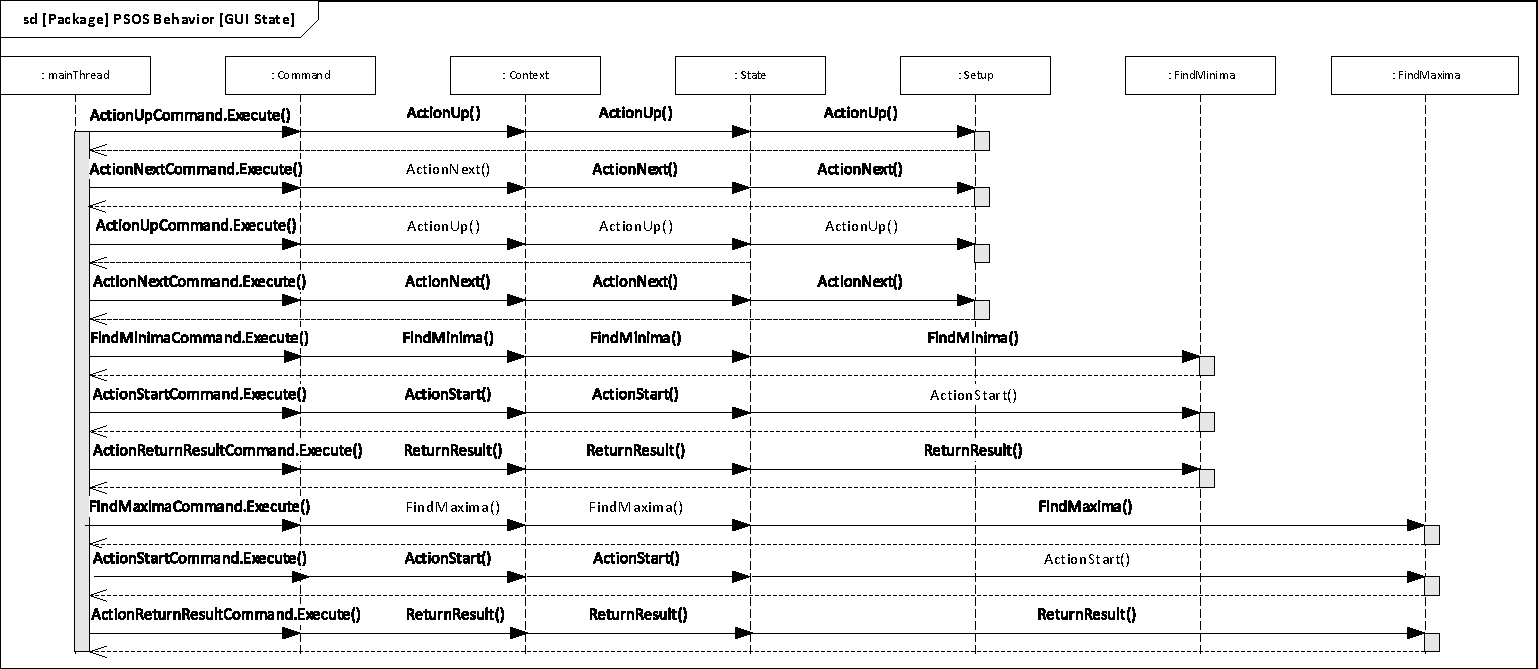
\includegraphics[width=1\linewidth]{diagram/sd_psos}
	\caption{Sequence Diagram for PSOS}
	\label{fig:sdpsos}
\end{figure}



\subsubsection{State Machine Diagram}\label{req:smd}

\begin{figure}[H]
	\centering
	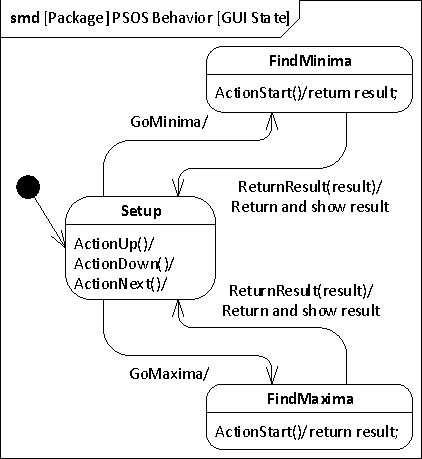
\includegraphics[width=0.7\linewidth]{diagram/smd_gui_state}
	\caption{State Machine Diagram of the Graphical User Interface}
	\label{fig:smdguistate}
\end{figure}
